\chapter{API Documentation}
Le API Locali fornite dall'applicazione Sistema Monitoraggio Ambientale e precedentemente descritte sono state documentate mediante il modulo NodeJS chiamato \texttt{Swagger-UI-Express}. Abbiamo definito le API utilizzando \texttt{JSDoc}, uno strumento volto alla generazione della documentazione utilizzando i commenti nel codice sorgente di un'applicazione. Così facendo la documentazione inerente alle API è visibile a chiunque visualizzi il codice sorgente. Per generare l'endpoint, la cui funzione è quella di presentare le API, abbiamo usato \texttt{Swagger UI} che genera una pagina web dalle definizioni delle specifiche OpenAPI.

\vspace{5mm}
\noindent
Di seguito mostriamo la pagina web contenente la documentazione che presenta le 15 API (di tipo GET, POST, PUT and DELETE) per la gestione dei dati nel nostro applicativo.

\vspace{5mm}
\noindent
La GET viene utilizzata per ottenere e visualizzare i dati in una pagina HTML. La POST serve ad inserire un nuovo dato nel sistema, la PUT modifica un dato presente nel sistema e la DELETE ne cancella uno.

\vspace{5mm}
\noindent
Dopo aver correttamente avviato le API mediante terminale, l'endpoint da invocare per poter visualizzare la seguente documentazione è: \textbf{http://localhost:49146/api-docs}

\begin{figure}[ht]
    \centering
    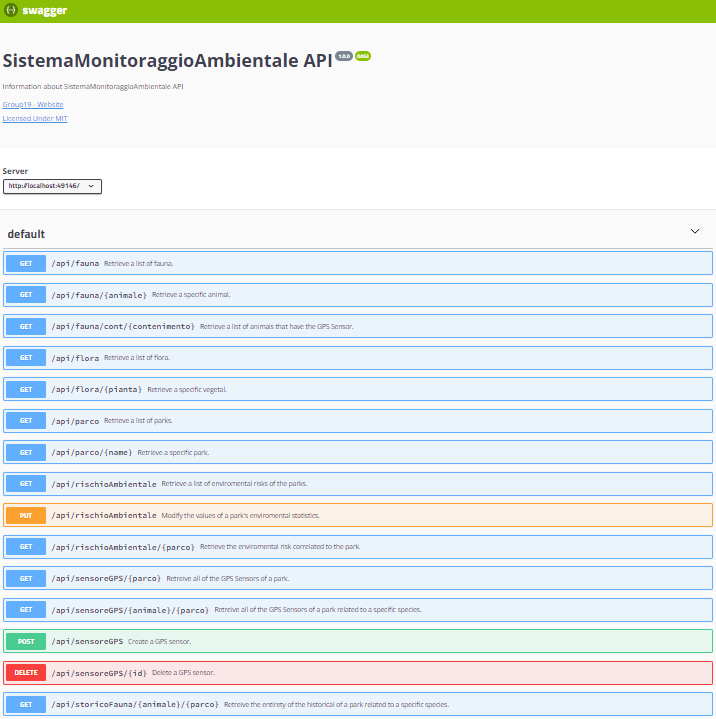
\includegraphics[scale=0.8]{Img/swagger.png}
    \caption{Documentazione delle API di Sistema di Monitoraggio Ambientale}
    \label{swagger}
\end{figure}